% Manuscript: local steering for rigid multi-robot payload transport.
% Build:  cd docs/paper && latexmk -pdf main.tex
% Tables and quoted numbers come from tools/make_paper_tables.py (never typed by hand).
\documentclass[journal]{IEEEtran}
\usepackage[utf8]{inputenc}
\usepackage[T1]{fontenc}
\usepackage{amsmath,amssymb}
\usepackage{graphicx}
\usepackage{booktabs}
\usepackage{adjustbox}
\usepackage{xcolor}
\usepackage{tikz}
\usetikzlibrary{arrows.meta,positioning,shapes.geometric,calc}
\usepackage[hidelinks]{hyperref}
\usepackage{cite}
\graphicspath{{../../results/figures_signals/}{../../results/figures_ext/}{../figures/}}
\newcommand{\XsAgree}{221}
\newcommand{\XsCells}{221}
\newcommand{\XcMax}{7\times10^{-7}}
\newcommand{\MpcContactNom}{19}
\newcommand{\MpcContactPhase}{47}
\newcommand{\MpcReachNom}{98}
\newcommand{\MpcReachPhase}{86}
\newcommand{\EnnReach}{90}
\newcommand{\EnnN}{90}
\newcommand{\EnoReach}{89}
\newcommand{\PavfhMs}{0.77}
\newcommand{\MpcMs}{2.46}
\newcommand{\PavfhTime}{90.3}
\newcommand{\MpcTime}{74.7}
\newcommand{\EzeroRej}{+0.12~[-2.71,~+3.00]}
\newcommand{\EzeroRejV}{inconclusive}
\newcommand{\EzeroTime}{-0.97~[-1.66,~-0.33]}
\newcommand{\EzeroTimeV}{improved}
\newcommand{\EzeroCon}{+0.17~[-0.93,~+1.19]}
\newcommand{\EzeroConV}{inconclusive}
\newcommand{\EzeroN}{360}
\newcommand{\EzeroReachNN}{351}
\newcommand{\EzeroReachNo}{351}
\newcommand{\EpoolRej}{-3.77~[-12.95,~+1.76]}
\newcommand{\EpoolRejV}{inconclusive}
\newcommand{\EpoolTime}{-0.95~[-1.53,~-0.38]}
\newcommand{\EpoolTimeV}{improved}
\newcommand{\EpoolCon}{+0.07~[-0.84,~+0.95]}
\newcommand{\EpoolConV}{inconclusive}
\newcommand{\EpoolN}{450}
\newcommand{\EpoolReachNN}{441}
\newcommand{\EpoolReachNo}{440}
\newcommand{\RoneSame}{90}
\newcommand{\RoneN}{90}
\newcommand{\RtwoClean}{9}
\newcommand{\RtwoN}{10}
\newcommand{\WdDelay}{0.3}
\newcommand{\PavfhPone}{0/20}
\newcommand{\PavfhPthree}{16/20}
\newcommand{\PavfhPfour}{22/40}
\newcommand{\MpcPfour}{39/40}
\newcommand{\NnPfour}{38/40}

\newcommand{\pavfh}{PA-VFH}
\definecolor{acc}{HTML}{2A78D6}
\definecolor{learn}{HTML}{D7E6FB}
\definecolor{safe}{HTML}{FBE3E1}
\definecolor{box}{HTML}{E9EEF7}

\begin{document}

\title{Steering a Rigid Multi-Robot Payload Through Dynamic Warehouses:\\
A Replicated Benchmark from Kinematics to Physics and ROS~2,\\
and a Hybrid Planner with Learned Occupancy Prediction}

\author{Authors~to~be~completed% TODO(authors): names, affiliations (Amrita), ORCIDs
\thanks{Code, scenarios, trained weights and every run are released with
SHA-256 checksums (archive DOI to be added).}}

\markboth{Draft manuscript}{Local steering for rigid multi-robot payload transport}

\maketitle

\begin{abstract}
Teams of mobile robots that carry one rigid payload must steer the whole
formation through clutter and moving traffic, yet their local steering laws
are rarely compared under a protocol that is reproducible, fair and carried
through to physics. We present an open benchmark in which twelve steering
laws---potential fields, VFH variants, the follow-the-gap method, DWA, a
lattice MPC, MPPI, an imitation-learned policy, and a new hybrid, \pavfh{}---move
formations of three to nine differential-drive robots through eight warehouse
layouts of up to 80\,$\times$\,50\,m. Two independent implementations
(MATLAB and Python) agree to $\XcMax$\,m at zero noise and in
\XsAgree{} of \XsCells{} cells of a 2{,}730-run noisy grid, after a
collision-test defect we found is corrected. Randomising the moving-traffic
phase roughly doubles every planner's contact rate (MPC: \MpcContactNom\,\% to
\MpcContactPhase\,\% of runs): a fixed timetable flatters all of them. We tune
every planner under the same budget, separate ground-truth collision screening
from deployable sensor-based and conformally calibrated learned monitors, and
replicate the physics study in MuJoCo through ROS~2 Humble, where all
\RoneN{} lockstep runs equal their in-process counterparts and the full
deployment stack, driven only by the robots' laser scans, completes
\RtwoClean{} of \RtwoN{} real-time missions without contact. \pavfh{} keeps a
classical VFH+ decision layer and learns only a small circular CNN that
predicts per-sector danger 0.5\,s ahead from the robots' own scans. In a
pre-registered confirmation on \EzeroN{} fresh paired missions, the network
shortened missions by about 1\,s (1\,\%; 95\,\% CI 0.3--1.7\,s) relative to its
non-learned twin, with no measurable change in gate rejections, contacts or
reach. \pavfh{} had the highest reach of the five laws compared at a third of
MPC's compute; MPC remained faster and more robust to robot-model mismatch.
All results are simulated.
\end{abstract}

\begin{IEEEkeywords}
Multi-robot systems, cooperative transport, local planning, benchmarking,
replication, learned occupancy, conformal prediction, MuJoCo, ROS~2.
\end{IEEEkeywords}

% =====================================================================
\section{Introduction}
\IEEEPARstart{C}{ooperative} payload transport lets several small mobile
robots move an object none of them could carry
alone~\cite{tuci2018,alonsomora2017,wang2016}. Once the robots have formed up
under the load, the team behaves as one rigid body: it must be steered as a
whole, its footprint rotates with its heading, and it shares the floor with
traffic that does not give way. The \emph{local steering law}---the component
that turns sensor data into a heading at 10\,Hz---decides whether the mission
succeeds and how safely.

Many such laws exist, from potential fields~\cite{khatib1986} and vector field
histograms~\cite{borenstein1991,ulrich1998} to the dynamic window
approach~\cite{fox1997}, model predictive control and its sampling variant
MPPI~\cite{williams2016,williams2018}, and, increasingly, learned policies.
They are, however, almost always evaluated one at a time, for single robots,
in a handful of scenarios, with whatever safety assumptions the authors'
simulator provides. Reproducibility is a recognised problem in learned
control~\cite{henderson2018,bettini2024}, and navigation benchmarks exist for
single robots~\cite{perille2020}, but none addresses a rigid multi-robot
payload among moving traffic, and none carries the comparison from
kinematics to physics and to a robot middleware.

This paper started as the proposal of a new histogram law and became, after
review and extended experiments, a benchmark-and-method paper. Its first
contribution is knowing \emph{how much} each design choice matters under a
protocol that flatters no one; its second is a hybrid that uses a neural
network where it is defensible, together with an honest measurement of what the
network adds. Concretely:

\begin{enumerate}
\item \textbf{A replicated, fair benchmark.} Two independent stacks agree
step for step; a defect in the reference collision test was found and fixed;
traffic phase is randomised; all laws use common random numbers, the same
tuning budget, held-out worlds and seeds; every failed run is reported with
95\,\% intervals.
\item \textbf{Evidence on what matters.} The per-beam range filter, not the
uncertainty-aware kernel, carries noise robustness; a fixed traffic timetable
hides half of all contacts; corridor width relative to the payload's swept
diameter, not robot count, limits the team; physics exposes clearance-hugging
behaviour that kinematics hides, and a uniform physical margin repairs most of it.
\item \textbf{Safety screening separated from monitoring}: a ground-truth
gate (simulator only), a geometric scan monitor and a learned monitor with a
split-conformal margin, each scored for false accepts.
\item \textbf{\pavfh{}}, a hybrid that learns only the occupancy prediction
inside an auditable VFH+ pipeline, from the robots' own scans, evaluated against
its own non-learned ablation in an exploratory and a pre-registered confirmatory
experiment; and a team-size-agnostic DAgger policy as the
end-to-end learned baseline.
\item \textbf{A path to deployment}: a ROS~2 package that reproduces the
MuJoCo missions exactly over DDS, drives real-time physics from laser scans,
and includes a safety watchdog; and a sensor-accuracy requirement derived from
the experiments.
\end{enumerate}

% =====================================================================
\section{Related Work}
\textit{Local steering.} Potential fields~\cite{khatib1986} react fast but
have local minima. VFH~\cite{borenstein1991} and VFH+~\cite{ulrich1998} build
a polar obstacle histogram and choose a free valley; VFH+ enlarges obstacles by
the body radius and adds hysteresis. Follow-the-gap~\cite{sezer2012} steers
into the widest gap. DWA~\cite{fox1997} searches reachable velocities.
MPPI~\cite{williams2016,williams2018} samples control sequences and is now a
default local controller family in ROS~2 navigation~\cite{macenski2020}.
These are rarely evaluated for a rigid multi-robot block.

\textit{Cooperative transport.} Reviews~\cite{tuci2018} cover force-based,
caging and formation approaches. Alonso-Mora \emph{et al.}~\cite{alonsomora2017}
plan formations around dynamic obstacles by constrained optimisation; Wang and
Schwager~\cite{wang2016} coordinate through the object without communication.
Transport papers usually couple the mission logic to the proposed planner, so
the planner's contribution cannot be isolated; here the mission layer is shared.

\textit{Learning and benchmarks.} Imitation learning with dataset aggregation
(DAgger)~\cite{ross2011}, permutation-invariant set encoders~\cite{zaheer2017}
and privileged-information training~\cite{chen2020} underlie our learned
components. Multi-agent benchmarks~\cite{bettini2022,bettini2024} standardise
tasks and reporting; navigation benchmarks~\cite{perille2020} do so for single
robots.

\textit{Safety.} Separating-axis tests~\cite{gottschalk1996} check convex
bodies exactly. Barrier functions~\cite{ames2019} and learned
certificates~\cite{dawson2023} give guarantees under model assumptions;
conformal prediction~\cite{vovk2005,angelopoulos2021} has been used for safe
planning among uncertain agents~\cite{lindemann2023}. Simulation studies often
report safety from the simulator's ground truth, which a robot does not have;
we measure that metric and deployable monitors separately.

% =====================================================================
\section{Problem and System}

\begin{figure}[t]
\centering
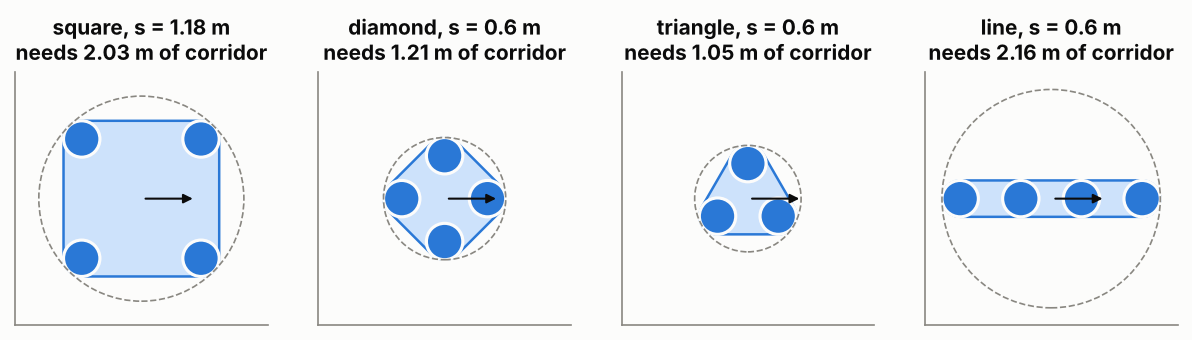
\includegraphics[width=0.92\columnwidth]{concept_formations.png}
\caption{Formation shapes. Disks are robots; the shaded region is the body
used by the collision test (convex hull of the slots grown by the robot
radius $r$); the dashed circle is the circumscribed circle, whose diameter is
the corridor width a rotating body can need.}
\label{fig:formations}
\end{figure}

\textit{Robots and formation.} $K$ differential-drive robots of radius
$r=0.18$\,m follow the unicycle model
\begin{align}
\theta_{k+1}&=\theta_k+\mathrm{clip}(\Delta\theta,\pm\omega_{\max}),\\
\mathbf{p}_{k+1}&=\mathbf{p}_k+v\,[\cos\theta_{k+1},\ \sin\theta_{k+1}]^\top \Delta t,
\end{align}
with $\Delta t=0.1$\,s. A mission has three phases: \emph{forming} (slots
assigned by minimum total travel~\cite{kuhn1955,crouse2016}, each robot steering
to its slot), \emph{docking}, and \emph{rigid transport}, in which robot $i$
occupies $\mathbf{c}+R(\theta)\,\mathbf{o}_i$ for a virtual leader
$(\mathbf{c},\theta)$ and fixed offsets $\mathbf{o}_i$. Shapes range from a
triangle ($K{=}3$) to a 3$\times$3 grid ($K{=}9$); Fig.~\ref{fig:formations}.

\textit{Traffic.} Movers are kinematic shuttles on piecewise-linear routes
that pause at their ends and never yield. Their schedule is stored in a
\emph{traffic contract}; some laws read the movers' future from it, which a
deployed robot usually cannot.

\textit{Sensing.} A 288-beam 2-D lidar (or a 60$^\circ$ ToF fan) returns
ranges with Gaussian noise of standard deviation $\sigma_0$.

\textit{Mission layer.} Shared by all laws: the steering direction is blended
with the goal direction, low-pass filtered and rate limited; every candidate
pose passes a \emph{safety gate} before it is committed; an escape probe and an
anti-deadlock layer resolve blocking; optional load-carrying motion limits bound
speed and accelerations.

% =====================================================================
\section{Steering Laws}
Table~\ref{tab:laws} lists the twelve laws. They differ only in the steering
vector they return.

\begin{table}[t]
\centering
\caption{Steering laws, the mover information they use, and compute per
control step (E15, mean over 800 runs).}
\label{tab:laws}
\adjustbox{max width=\columnwidth}{\footnotesize
\setlength{\tabcolsep}{3pt}
\begin{tabular}{lllr}
\toprule
Law & Mechanism & Mover information & ms/step \\
\midrule
VFH & histogram & predicted scan & 0.91 \\
FGM & gap & predicted scan & 1.70 \\
DWA & velocity sampling & predicted scan & 2.05 \\
MPC & lattice MPC & predicted scan & 3.89 \\
MPPI & sampling MPC & predicted scan & 5.90 \\
pVFH & histogram + horizon & contract & 2.04 \\
PA-VFH-K & + range filter + kernel & contract & 1.88 \\
NN (DAgger) & learned policy (DAgger) & predicted scan & 1.76 \\
PA-VFH (no NN) & + range filter + kernel & \textbf{own scans only} & 0.71 \\
\textbf{PA-VFH} & + range filter + learned occupancy & \textbf{own scans only} & 0.85 \\
\bottomrule
\end{tabular}
}
\end{table}

\textit{Histogram family.} A scan is binned into $S=72$ sectors of 5$^\circ$.
With $d_s$ the nearest return in sector $s$, the danger is
\begin{equation}
u_s=\exp\!\left(-d_s^2/2\sigma_h^2\right),
\end{equation}
with $\sigma_h$ set so that $u_s$ crosses the threshold $\tau=0.3$ at the body
radius plus a reaction gap. VFH+ enlargement marks every sector within
$\gamma=\arcsin(r_b/d_s)$ of an obstacle; after circular smoothing the law picks
the free sector closest to the goal, with a hysteresis penalty, and adds a
short-range repulsion. The ablation ladder adds one ingredient at a time: the
movers' predicted positions (pVFH), a per-beam Kalman range
filter~\cite{kalman1960} (pVFH+F),
\begin{equation}\small
K=\frac{P+q^2}{P+q^2+s^2},\ \ x\leftarrow x+K(z-x),\ \ P\leftarrow(1-K)(P+q^2),
\end{equation}
reset when $|z-x|>3\sqrt{P+q^2+s^2}$, and finally the posterior-expected
kernel (PA-VFH-K, the original proposal),
\begin{equation}
\mathbb{E}[u]=\sqrt{\frac{\sigma_h^2}{\sigma_h^2+s^2}}\exp\!\left(-\frac{d^2}{2(\sigma_h^2+s^2)}\right).
\end{equation}

\textit{External baselines.} APF, FGM, DWA, a lattice MPC that scores a tree
of heading changes with a soft safety distance $d_{\mathrm{safe}}$, and MPPI with
$N=256$ samples weighted by $\exp(-J/\lambda)$.

\textit{Learned baseline.} The DAgger policy~\cite{ross2011} imitates MPC.
It encodes the scan with a circular 1-D CNN and the slots with a DeepSets
encoder~\cite{zaheer2017}, so one network serves any team size.

\begin{figure*}[t]
\centering
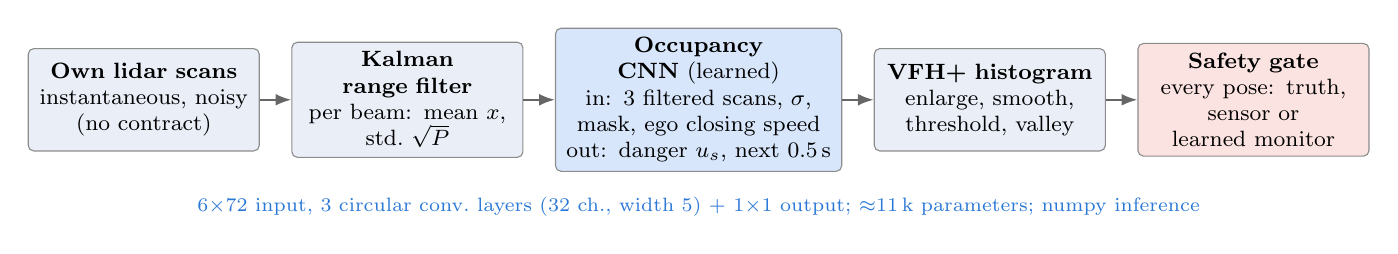
\begin{tikzpicture}[
  node distance=4mm,
  blk/.style={draw=black!45, rounded corners=2pt, align=center, minimum height=13mm,
              text width=27mm, font=\footnotesize, fill=box},
  arr/.style={-{Latex[length=2mm]}, thick, black!60}]
\node[blk] (scan) {\textbf{Own lidar scans}\\instantaneous, noisy\\(no contract)};
\node[blk, right=of scan] (kf) {\textbf{Kalman range filter}\\per beam: mean $x$,\\std.\ $\sqrt{P}$};
\node[blk, right=of kf, fill=learn, text width=34mm] (nn) {\textbf{Occupancy CNN} (learned)\\in: 3 filtered scans, $\sigma$,\\mask, ego closing speed\\out: danger $u_s$, next 0.5\,s};
\node[blk, right=of nn] (hist) {\textbf{VFH+ histogram}\\enlarge, smooth,\\threshold, valley};
\node[blk, right=of hist, fill=safe] (gate) {\textbf{Safety gate}\\every pose: truth,\\sensor or learned monitor};
\draw[arr] (scan)--(kf); \draw[arr] (kf)--(nn); \draw[arr] (nn)--(hist); \draw[arr] (hist)--(gate);
\node[below=2mm of nn, font=\scriptsize, text=acc, align=center] {6$\times$72 input, 3 circular conv.\ layers (32 ch., width 5) + 1$\times$1 output; $\approx$11\,k parameters; numpy inference};
\end{tikzpicture}
\caption{\pavfh{}. Only the danger prediction is learned; the decision layer
and the gate stay classical. The network is trained against oracle labels that
use the movers' true future but, at run time, sees only the robots' scans.}
\label{fig:pavfh}
\end{figure*}

\subsection{\pavfh{}: VFH+ with Learned Occupancy}
\pavfh{} (Fig.~\ref{fig:pavfh}) addresses two findings about its predecessor:
the uncertainty-aware kernel had almost no effect, and the law read the
movers' future from the contract. \pavfh{} uses only the robots' instantaneous
scans. Its input is a $6\times72$ tensor: the sector minimum range minus the
body radius for the last three filtered scans, the posterior $\sigma$, an
observed mask and the formation's closing speed toward each sector. A fully
convolutional, circular network (equivariant to rotations by whole sectors)
outputs $u_s\in(0,1)$, which replaces the analytic kernel; everything after it
is unchanged. Labels are the danger an oracle computes from the \emph{true}
sector minimum over the next 0.5\,s---privileged information available only in
simulation~\cite{chen2020}. Training uses soft-label binary cross-entropy with
dangerous sectors up-weighted, and two rounds: data collected while the
non-learned pipeline drives, then on-policy while \pavfh{} drives. Training
worlds and seeds are disjoint from the evaluation ones.

% =====================================================================
\section{Safety: Screening Versus Monitoring}
\textit{Ground-truth gate.} The gate checks the body at $t$ and $t+\Delta t$
against statics and movers with an exact separating-axis test~\cite{gottschalk1996}.
The reference implementation listed box corners as $(+,+),(+,-),(-,+),(-,-)$; this
order is not cyclic, so one box normal was never tested and some clear poses
were rejected. The defect is conservative but inflated rejections; we fixed it
in both stacks. In simulation the gate is a \emph{screening device}: it
measures what a law asks for while an oracle prevents static collisions.

\textit{Deployable monitors.} The geometric monitor admits a pose only if every
filtered scan point clears the body by $r+k\sigma+v_{\mathrm{obs}}h$
($k=3$, $v_{\mathrm{obs}}=1$\,m/s, $h=0.2$\,s). The learned monitor regresses
the clearance $\hat c$ and admits iff $\hat c-q_\alpha>r$, where $q_\alpha$ is
the $\lceil(n+1)(1-\alpha)\rceil$-th smallest calibration residual---a split
conformal margin~\cite{vovk2005,angelopoulos2021} whose guarantee is marginal and
in-distribution. In \emph{audit} mode the truth decides and a monitor is scored
in its shadow. A false accept is a pose a monitor admits that the truth rejects.

% =====================================================================
\section{Benchmark Protocol}
\textit{Randomness.} All laws in a cell share seeds (common random numbers).
Each seed also draws mover start offsets from an independent stream, so the
traffic phase varies per run while geometry is unchanged. Evaluation uses seeds
1--10; training and tuning use seeds $\geq101$.

\textit{Tuning.} Every law gets 24 configurations (its defaults included) on the
same seven training missions; default and tuned laws are then compared on ten
held-out worlds (E18).

\textit{Experiments.} The replicated grid (E1--E14, 2{,}730 runs per stack);
layouts E15 (8 warehouses, 800 runs); team size E16 (3--9 robots, 900 runs);
monitors E17 (816 runs); tuning E18 (700 runs); the \pavfh{} ablation E19 (450
runs); MuJoCo physics~\cite{todorov2012} P1--P4 (720 runs); and ROS~2
physics R1--R2 (100 runs).

\textit{Statistics.} Rates carry Wilson 95\,\% intervals~\cite{wilson1927};
means carry 2{,}000-sample percentile-bootstrap intervals~\cite{efron1979};
paired differences use common-random-number pairs. Every failed run counts.

% =====================================================================
\section{Results}

\subsection{Replication}
Table~\ref{tab:repl} and Fig.~\ref{fig:xstack}. At zero noise the two stacks
take identical steps for every law; in the noisy grid all cells agree once the
gate is corrected. Matching tie-breaking in the slot assignment required porting
the same shortest-augmenting-path solver~\cite{crouse2016} to the reference.

\begin{table}[t]
\centering
\caption{MATLAB vs.\ Python with the corrected collision gate.}
\label{tab:repl}
\adjustbox{max width=\columnwidth}{\footnotesize
\setlength{\tabcolsep}{3pt}
\begin{tabular}{lp{0.58\columnwidth}}
\toprule
Check & Result \\
\midrule
Zero noise, step by step (8 laws) & max centroid diff.\ 7.0e-07 m; never $>$1 mm \\
Noisy grid, cells agreeing & 221/221 \\
Correlation of cell means & time 0.981, rejections 0.949, gap 0.990 \\
Runs reaching the goal & MATLAB 2605/2730, Python 2621/2730 \\
Static-contact steps & 0 in both stacks \\
\bottomrule
\end{tabular}
}
\end{table}

\begin{figure*}[t]
\centering
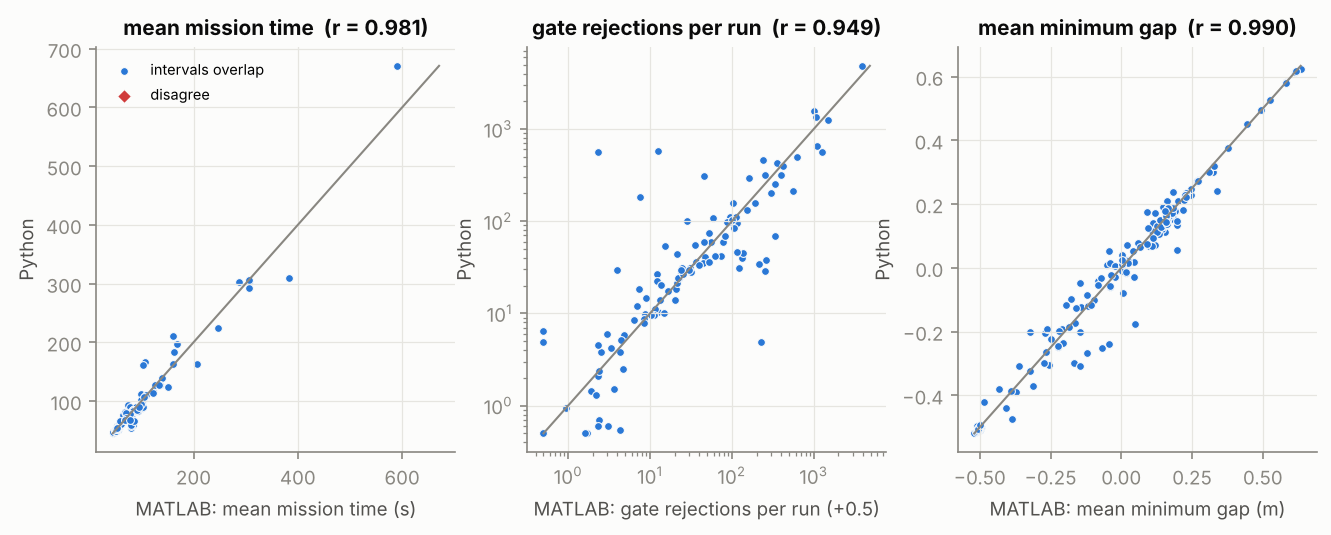
\includegraphics[width=0.95\textwidth]{cross_stack_scatter_fixedgate.png}
\caption{Cross-stack agreement over the 2{,}730-run grid. Each dot is an
experiment cell (x: MATLAB mean, y: Python mean). Blue: 95\,\% intervals
overlap; all \XsAgree{} cells agree.}
\label{fig:xstack}
\end{figure*}

\subsection{What Carries Noise Robustness}
Along the ablation ladder (Fig.~\ref{fig:e2}), adding the mover horizon changes
nothing; adding the range filter flattens time and rejections against
$\sigma_0$; adding the expected kernel changes nothing measurable. Analytically,
at $\sigma_0\le0.4$\,m the kernel moves the reaction distance by about 3\,\%.

\begin{figure*}[t]
\centering
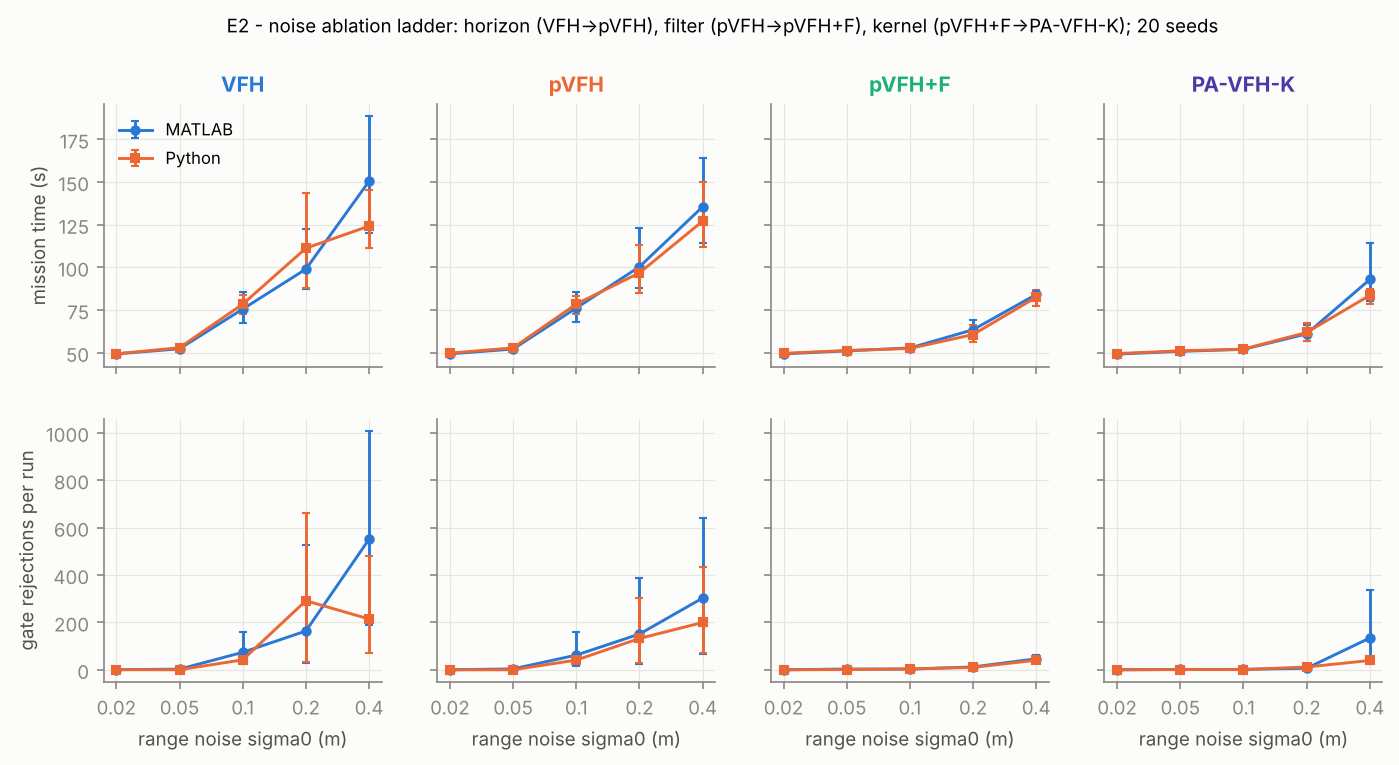
\includegraphics[width=0.95\textwidth]{e2_noise_both_stacks_fixedgate.png}
\caption{Ablation ladder against sensor noise (both stacks). The range filter
(pVFH$\to$pVFH+F) is the effective ingredient; the expected kernel
(pVFH+F$\to$PA-VFH-K) adds nothing measurable.}
\label{fig:e2}
\end{figure*}

\subsection{A Fixed Timetable Flatters Every Planner}
Randomising the traffic phase (Table~\ref{tab:phase}, Fig.~\ref{fig:phase})
raises the share of runs with contact for every law and lowers reach; MPC goes
from \MpcContactNom\,\% to \MpcContactPhase\,\% contact runs and from
\MpcReachNom\,\% to \MpcReachPhase\,\% reach. Rankings from a single timetable
should not be trusted.

\begin{table}[t]
\centering
\caption{Nominal timetable vs.\ randomised traffic phase, pooled grid.}
\label{tab:phase}
\adjustbox{max width=\columnwidth}{\footnotesize
\setlength{\tabcolsep}{3pt}
\begin{tabular}{lrrrrr}
\toprule
Law & Reach nom. & Reach rand. & Contact nom. & Contact rand. & $n$ \\
\midrule
VFH & 97\,\% & 90\,\% & 39\,\% & 53\,\% & 410 \\
FGM & 87\,\% & 83\,\% & 35\,\% & 37\,\% & 150 \\
DWA & 96\,\% & 78\,\% & 26\,\% & 50\,\% & 320 \\
MPC & 98\,\% & 86\,\% & 19\,\% & 47\,\% & 320 \\
pVFH & 98\,\% & 88\,\% & 33\,\% & 46\,\% & 530 \\
pVFH+F & 97\,\% & 91\,\% & 26\,\% & 40\,\% & 320 \\
PA-VFH-K & 98\,\% & 88\,\% & 26\,\% & 48\,\% & 530 \\
\bottomrule
\end{tabular}
}
\end{table}

\begin{figure}[t]
\centering
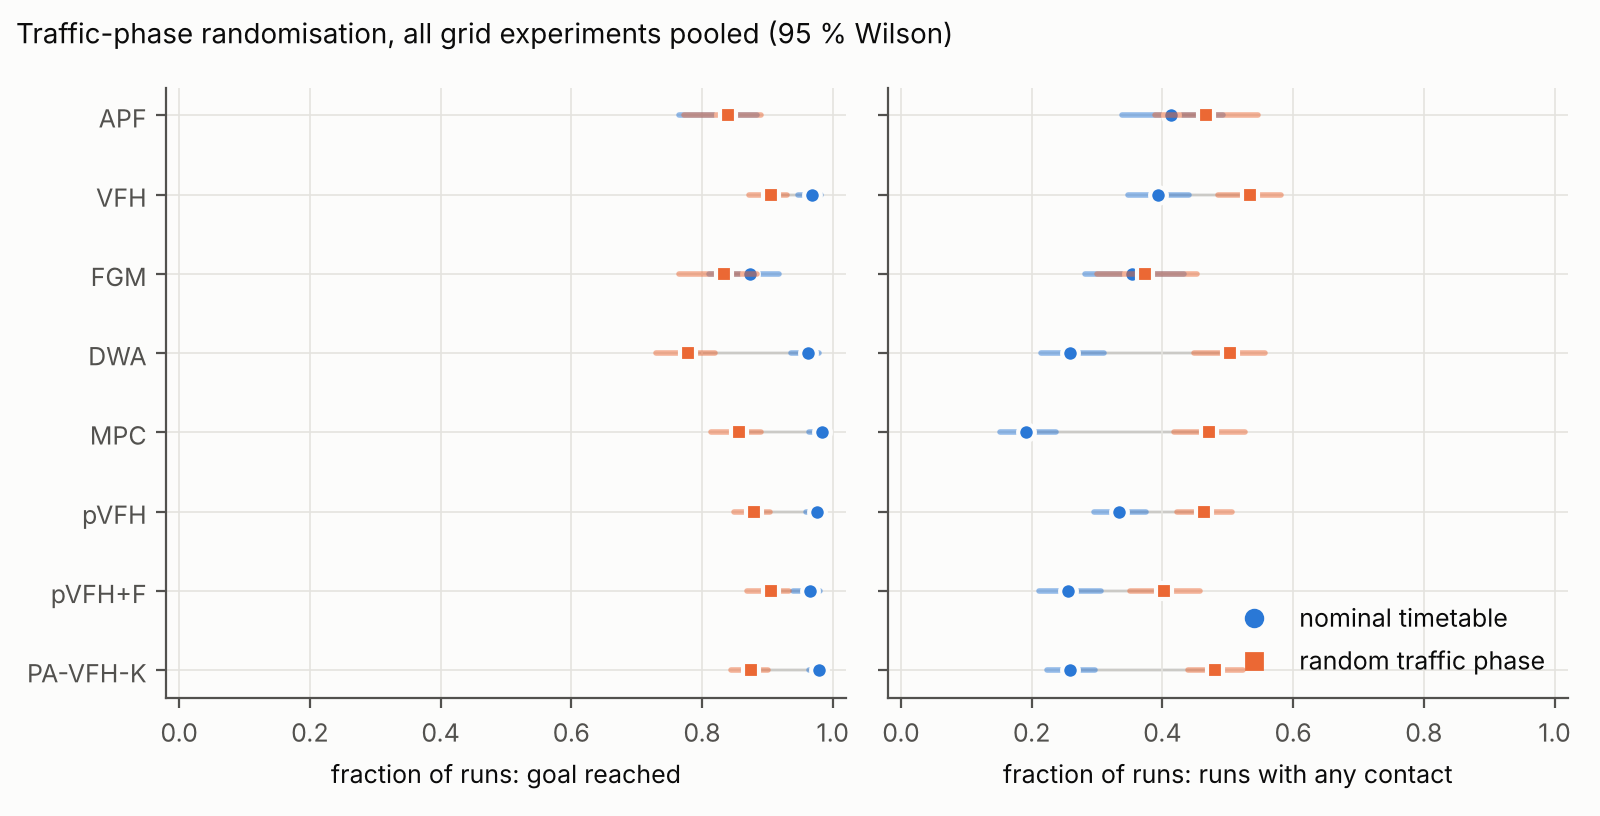
\includegraphics[width=\columnwidth]{fig_phase_effect.png}
\caption{Reach (left) and runs with any contact (right), nominal timetable
(circles) vs.\ random phase (squares), Wilson 95\,\% intervals.}
\label{fig:phase}
\end{figure}

\subsection{Layouts and Team Size}
Table~\ref{tab:layouts} and Fig.~\ref{fig:scale}. No law passes the narrow-aisle
warehouse (2.4\,m aisles). A 2$\times$2\,m nine-robot payload (swept diameter
$\approx$3.2\,m) fails in the study warehouse's 2.45\,m corridor for every law
but MPPI, yet passes in the large rack warehouses; nine robots under a small
payload are easy. Corridor width relative to the swept diameter, not robot
count, is the limit. \pavfh{} is tied for the highest reach in both E15 and E16.

\begin{table}[t]
\centering
\caption{E15 (8 layouts, 80 runs/law) and E16 (team sizes, 150 runs/law):
reached and runs with contact.}
\label{tab:layouts}
\adjustbox{max width=\columnwidth}{\scriptsize
\setlength{\tabcolsep}{3pt}
\begin{tabular}{lrrrr}
\toprule
Law & E15 reach & E15 contact & E16 reach & E16 contact \\
\midrule
VFH & 68/80 & 19/80 & -- & -- \\
FGM & 65/80 & 32/80 & -- & -- \\
DWA & 66/80 & 27/80 & 125/150 & 79/150 \\
MPC & 68/80 & 30/80 & 135/150 & 68/150 \\
MPPI & 68/80 & 31/80 & 138/150 & 73/150 \\
PA-VFH-K & 67/80 & 15/80 & 135/150 & 59/150 \\
NN (DAgger) & 69/80 & 29/80 & 128/150 & 61/150 \\
PA-VFH (no NN) & 68/80 & 18/80 & -- & -- \\
\textbf{PA-VFH} & 69/80 & 21/80 & 138/150 & 80/150 \\
\bottomrule
\end{tabular}
}
\end{table}

\begin{figure*}[t]
\centering
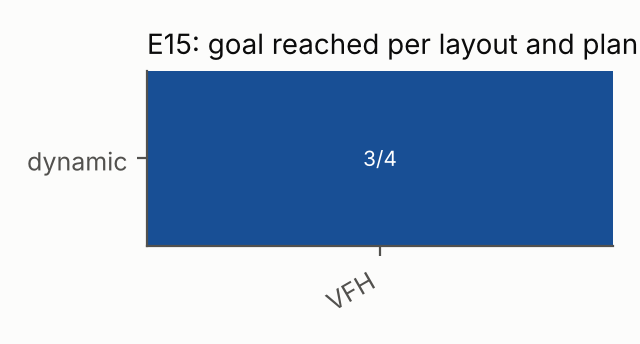
\includegraphics[height=4.4cm]{fig_e15_reach.png}\hfill
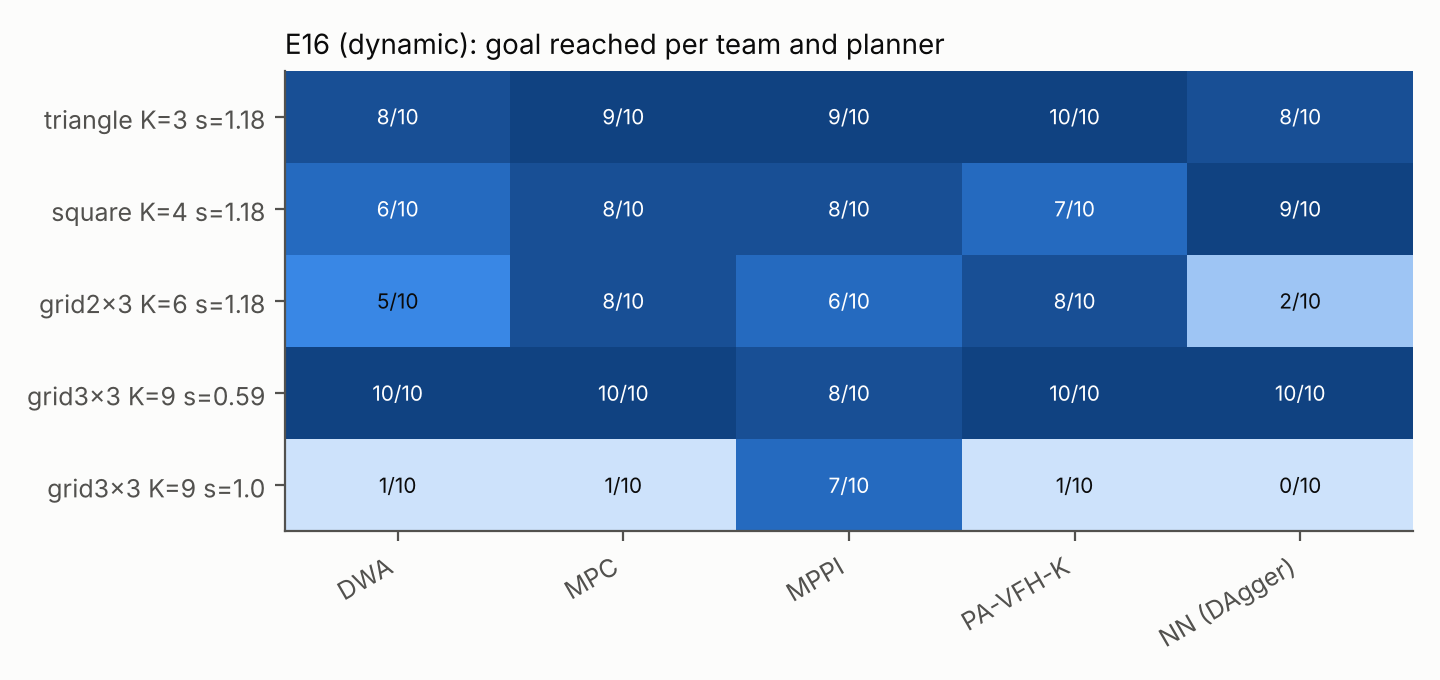
\includegraphics[height=4.4cm]{fig_e16_dynamic.png}
\caption{Left: E15 goal reached per layout and law. Right: E16 per team in the
study warehouse; the 3$\times$3 grid at $s=1.0$\,m fails for all laws but MPPI.}
\label{fig:scale}
\end{figure*}

\subsection{Deployable Safety}
Table~\ref{tab:mon} and Fig.~\ref{fig:mon}. The geometric monitor matches the
ground truth at $\sigma_0=0.02$\,m with no false accepts, but its $3\sigma$
inflation closes the corridors at $\sigma_0=0.10$\,m and reach collapses. The
learned monitor keeps reach at both noise levels but admits more unsafe poses.
Both deployable monitors see more contact runs than the ground truth; most are
movers driving into a formation that a pose check cannot protect.

\begin{table}[t]
\centering
\caption{E17: gate type, reach, contact runs and false accepts per 1000 gate
checks (240 runs per gate type).}
\label{tab:mon}
\adjustbox{max width=\columnwidth}{\scriptsize
\setlength{\tabcolsep}{3pt}
\begin{tabular}{lllll}
\toprule
Gate & $\sigma_0$ & Reach & Contact runs & FA/1000 \\
\midrule
Ground truth (audit) & 0.02 & 115/120 [0.91, 0.98] & 45/120 [0.29, 0.46] & -- \\
 & 0.10 & 116/120 [0.92, 0.99] & 44/120 [0.29, 0.46] & -- \\
Geometric sensor monitor & 0.02 & 119/120 [0.95, 1.00] & 66/120 [0.46, 0.64] & 0.00 \\
 & 0.10 & 63/120 [0.44, 0.61] & 81/120 [0.59, 0.75] & 0.00 \\
Learned + conformal ($\alpha{=}0.05$) & 0.02 & 116/120 [0.92, 0.99] & 67/120 [0.47, 0.64] & 2.88 \\
 & 0.10 & 112/120 [0.87, 0.97] & 76/120 [0.54, 0.71] & 5.37 \\
\bottomrule
\end{tabular}
}
\end{table}

\begin{figure*}[t]
\centering
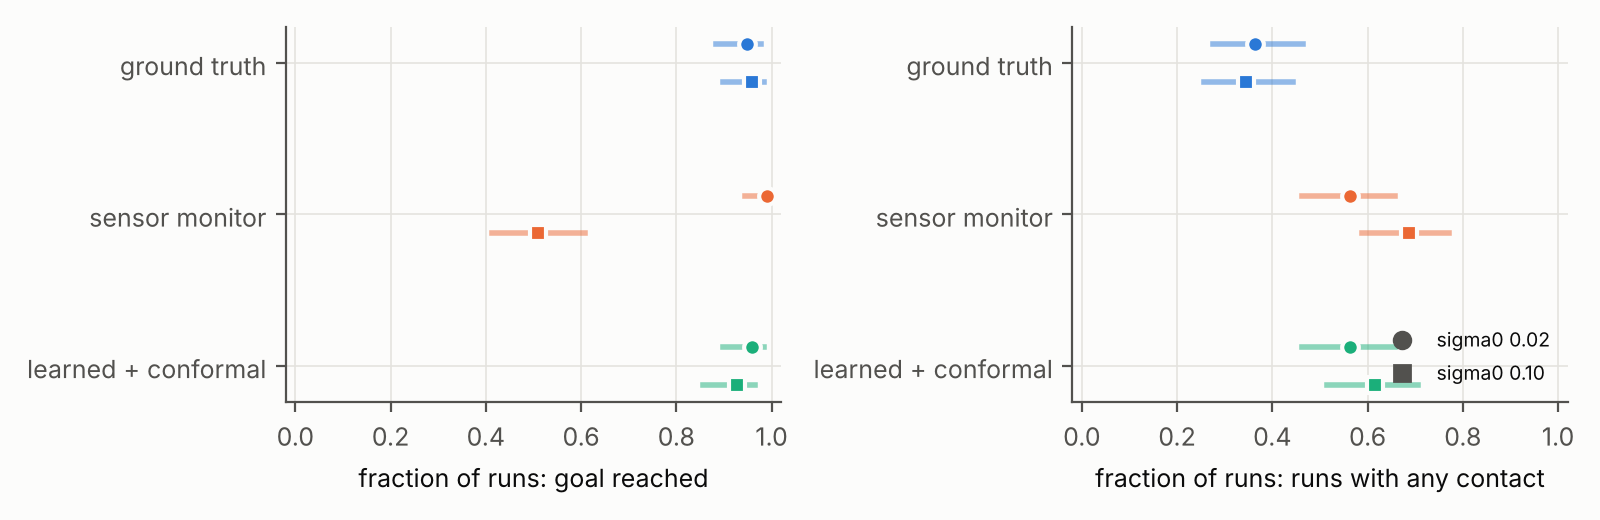
\includegraphics[height=3.7cm]{fig_e17_monitor.png}\hfill
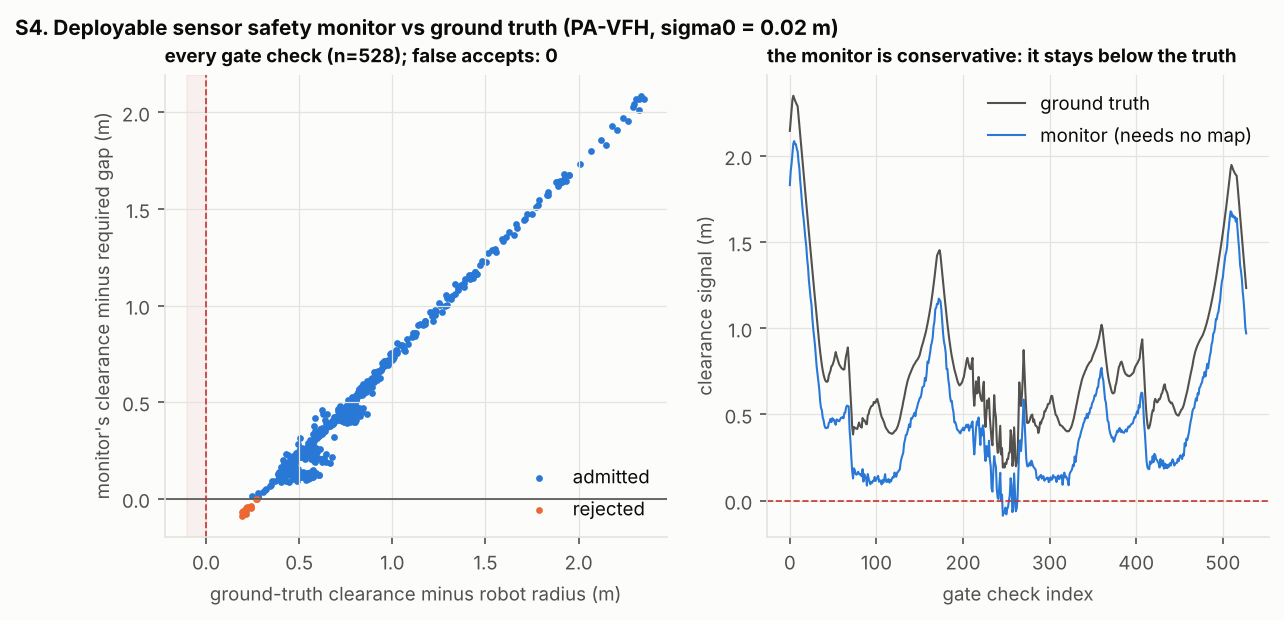
\includegraphics[height=3.7cm]{S4_monitor_signals.png}
\caption{Left: E17 reach and contact by gate type. Right: every gate check of
one mission with the sensor monitor deciding; a false accept would be a blue
point left of zero. The monitor stays below the truth.}
\label{fig:mon}
\end{figure*}

\subsection{Fair Tuning}
Under the equal budget, tuning improved the training objective for every law
(e.g.\ FGM 271\,$\to$\,97, DWA 89\,$\to$\,62, \pavfh{} 128\,$\to$\,96), but on
held-out worlds the paired cost change was near zero for most laws: the
defaults were not a straw man, and \pavfh{} did not gain from tuning that the
baselines lacked.

\subsection{Does the Network Help \pavfh{}?}
Table~\ref{tab:e19} compares \pavfh{} with its non-learned twin (same pipeline,
analytic kernel), with PA-VFH-K (which reads the contract), and with MPC and
MPPI. In E19 (90 pairs) the network completed one more mission and appeared to
halve gate rejections, but every paired interval included or touched zero. We
therefore ran a confirmatory experiment, E20, whose design and analysis were
fixed and committed before any run: \EzeroN{} new paired missions (seeds 7--30;
same worlds and noise levels; no retraining or tuning). Table~\ref{tab:e20}
gives the result. Mission time is \emph{improved}: \EzeroTime\,s per mission,
about 1\,\%, and the pooled 450-pair estimate agrees (\EpoolTime\,s). Gate
rejections (\EzeroRej) and contact steps (\EzeroCon) are inconclusive, and reach
is identical (\EzeroReachNN{} vs.\ \EzeroReachNo{}): the E19 reduction in
rejections came from a few long stalls and did not replicate. The network
therefore makes \pavfh{} slightly but measurably faster and is otherwise
neutral. At the signal level (Fig.~\ref{fig:s3}) the network agrees with
the oracle on blocked/free sectors slightly more often than the analytic kernel
(98.2\,\% vs.\ 98.0\,\%) and misses fewer blocked sectors, while its mean value
error is larger because it hedges on free sectors; it also over-predicts danger
before three frames of history exist. \pavfh{} has the highest reach of the five
laws at \PavfhMs\,ms per step versus \MpcMs\,ms for MPC; MPC is faster
(\MpcTime\,s vs.\ \PavfhTime\,s), and PA-VFH-K, which sees the movers' future,
has fewer contact runs.

\begin{table}[t]
\centering
\caption{E19 ablation (450 runs; 5 worlds $\times$ 3 noise levels $\times$ 6
seeds; random phase). Top: pooled per law. Bottom: paired differences.}
\label{tab:e19}
\adjustbox{max width=\columnwidth}{\scriptsize
\setlength{\tabcolsep}{3pt}
\begin{tabular}{llllll}
\toprule
Law & Reach & Contact runs & Time (s) & Rejections & ms \\
\midrule
\textbf{PA-VFH} & 90/90 [0.96, 1.00] & 32/90 [0.26, 0.46] & 90.3 [80.8, 101.4] & 19.6 [14.4, 25.6] & 0.77 \\
PA-VFH (no NN) & 89/90 [0.94, 1.00] & 31/90 [0.25, 0.45] & 91.4 [81.9, 102.3] & 38.9 [16.0, 79.8] & 0.64 \\
PA-VFH-K & 86/90 [0.89, 0.98] & 14/90 [0.09, 0.24] & 88.8 [81.1, 98.0] & 83.0 [27.6, 155.9] & 1.12 \\
MPC & 87/90 [0.91, 0.99] & 26/90 [0.21, 0.39] & 74.7 [69.2, 80.9] & 71.3 [13.3, 144.0] & 2.46 \\
MPPI & 86/90 [0.89, 0.98] & 30/90 [0.24, 0.44] & 79.1 [73.2, 85.6] & 100.9 [33.4, 187.6] & 4.06 \\
\bottomrule
\end{tabular}
}\\[2mm]
\adjustbox{max width=\columnwidth}{\footnotesize
\setlength{\tabcolsep}{3pt}
\begin{tabular}{ll}
\toprule
Paired PA-VFH $-$ PA-VFH (no NN) & Mean [95\,\% CI] \\
\midrule
Missions (paired) & 90 \\
Reached, network / no network & 90 / 89 \\
Time difference (s), both reached & -0.9 [-2.1, +0.2] \\
Rejected-step difference & -19.3 [-57.6, +0.7] \\
Contact-step difference & -0.3 [-1.9, +1.0] \\
\bottomrule
\end{tabular}
}
\end{table}

\begin{table}[t]
\centering
\caption{E20, pre-registered confirmation: paired difference \pavfh{} $-$
\pavfh{} (no NN) on identical missions; 95\,\% bootstrap intervals (10{,}000
resamples). ``Improved'': interval entirely below zero.}
\label{tab:e20}
\adjustbox{max width=\columnwidth}{\scriptsize
\setlength{\tabcolsep}{3pt}
\begin{tabular}{lllll}
\toprule
Set & Paired outcome (NN $-$ no NN) & Pairs & Mean [95\,\% CI] & Verdict \\
\midrule
E20 (confirmatory) & Rejected steps & 360 & +0.12 [-2.71, +3.00] & inconclusive \\
 & Time (s), both reached & 351 & -0.97 [-1.66, -0.33] & improved \\
 & Contact steps & 360 & +0.17 [-0.93, +1.19] & inconclusive \\
E19+E20 pooled & Rejected steps & 450 & -3.77 [-12.95, +1.76] & inconclusive \\
 & Time (s), both reached & 440 & -0.95 [-1.53, -0.38] & improved \\
 & Contact steps & 450 & +0.07 [-0.84, +0.95] & inconclusive \\
\bottomrule
\end{tabular}
}
\end{table}

\begin{figure}[t]
\centering
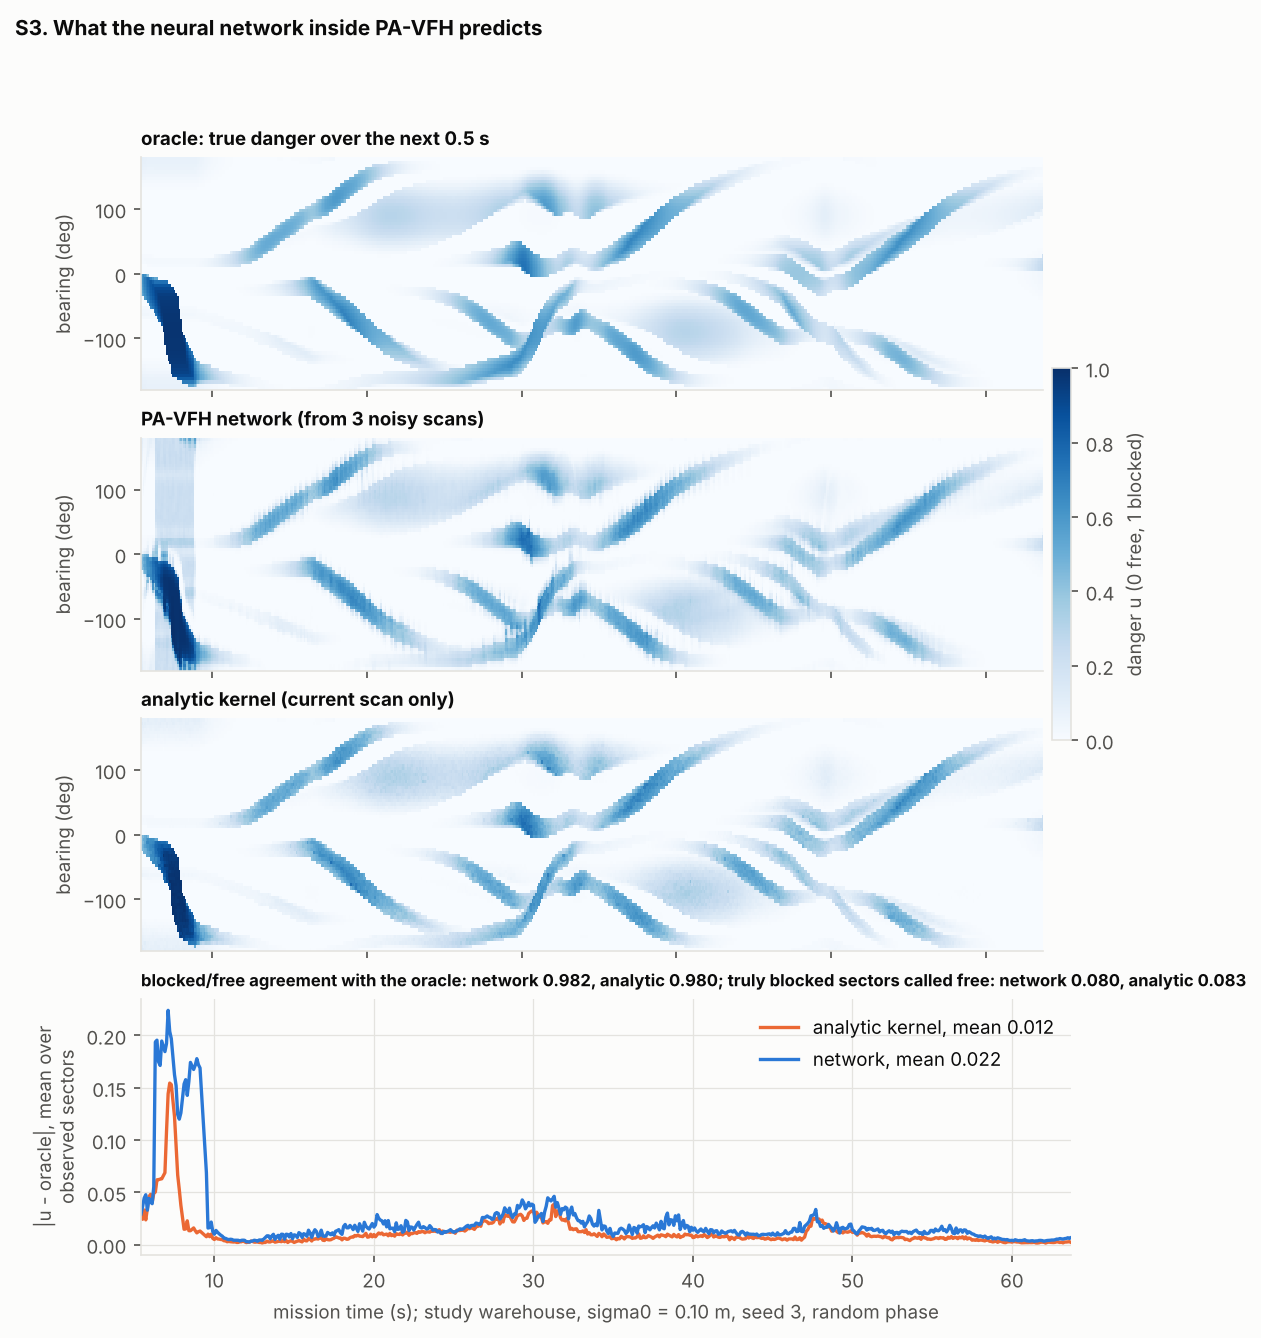
\includegraphics[width=\columnwidth]{S3_pavfh_danger_maps.png}
\caption{Inside \pavfh{} over one mission ($\sigma_0=0.10$\,m): oracle danger
(true future), the network's prediction, and the analytic kernel, per bearing
and time; bottom, the per-step error against the oracle.}
\label{fig:s3}
\end{figure}

\subsection{Physics}
In MuJoCo (pinned load, wheel slip, torque limits) the histogram laws first
grazed static racks in nearly every run (Table~\ref{tab:phys}, P1): they steer
to the smallest clearance the kinematic gate admits, about 1\,mm, which tracking
error consumes (Fig.~\ref{fig:s1}). A 0.10\,m clearance margin in the gate,
applied to every law, raised \pavfh{} from \PavfhPone{} to \PavfhPthree{} clean
runs with a carried or virtual load, while MPC---whose cost already keeps
$d_{\mathrm{safe}}$---was unaffected. Under robot-model mismatch (P4: mass,
wheel speed, friction, payload and motor force varied) \pavfh{} reached
\PavfhPfour{} clean runs versus \MpcPfour{} for MPC and \NnPfour{} for the
DAgger policy. A towed load swings outside the modelled footprint and defeats
every law.

\begin{table}[t]
\centering
\caption{Clean physics runs (reached, no contact in MuJoCo). P1: no margin;
P3/P4: 0.10\,m margin (P4: robot-parameter sweep); R1: P3 through ROS~2.
``Towed'': load pulled behind; other columns: carried and virtual load.}
\label{tab:phys}
\adjustbox{max width=\columnwidth}{\scriptsize
\setlength{\tabcolsep}{3pt}
\begin{tabular}{lrrrrrr}
\toprule
Law & P1 & P3 & P3 towed & P4 sweep & R1 (ROS\,2) & R1 towed \\
\midrule
\textbf{PA-VFH} & 0/20 & 16/20 & 0/10 & 22/40 & 8/10 & 0/5 \\
MPC & 20/20 & 20/20 & 2/10 & 39/40 & 10/10 & 2/5 \\
NN (DAgger) & 20/20 & 20/20 & 6/10 & 38/40 & 10/10 & 2/5 \\
MPPI & 15/20 & 15/20 & 0/10 & 34/40 & 10/10 & 0/5 \\
DWA & 18/20 & 18/20 & 0/10 & 30/40 & 10/10 & 0/5 \\
PA-VFH-K & 1/20 & 14/20 & 0/10 & 13/40 & 6/10 & 0/5 \\
\bottomrule
\end{tabular}
}
\end{table}

\begin{figure}[t]
\centering
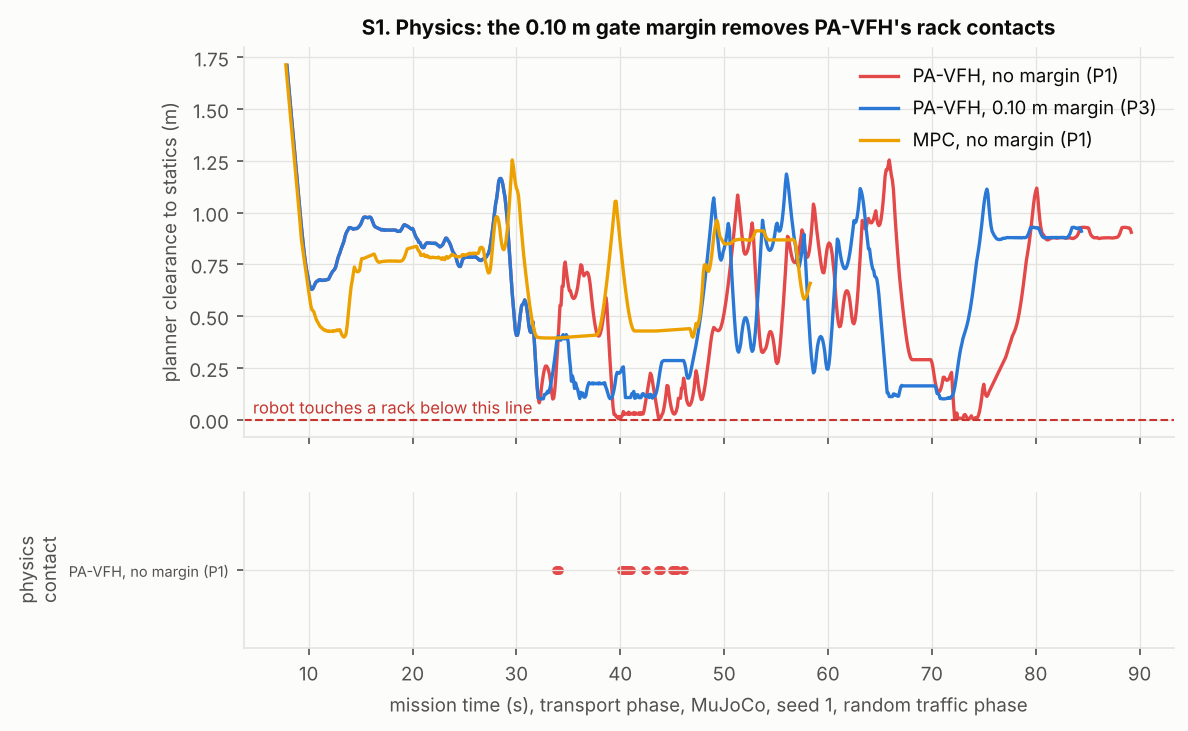
\includegraphics[width=\columnwidth]{S1_physics_margin_clearance.png}
\caption{Same MuJoCo mission without (red) and with (blue) the 0.10\,m margin,
and MPC (amber): clearance to statics; bottom, physical contacts.}
\label{fig:s1}
\end{figure}

\subsection{ROS~2 and Deployment}
The ROS~2 package (Humble) runs the MuJoCo plant and the controller as
separate nodes~\cite{macenski2022}. In lockstep over DDS, all \RoneN{} R1 runs
are identical on every metric to the in-process physics run in the same
environment (Fig.~\ref{fig:s5}); against a different MuJoCo version, chaotic
missions diverge from $\sim\!10^{-14}$ floating-point differences, so identity
must be checked within one environment. In the full deployment stack (R2) the
plant runs free, publishes odometry and 360-beam laser scans from the physical
robots, and the controller---\pavfh{}, the sensor monitor, a watchdog and the
0.10\,m margin---sees only those scans: \RtwoClean{} of \RtwoN{} real-time
missions finished with no physical contact; the tenth was struck by a shuttle.
When a robot's lidar stopped, the watchdog raised the safety flag after
\WdDelay\,s and every robot stopped. Running the controller on simulation time
was necessary whenever the simulator fell behind real time.

\begin{figure}[t]
\centering
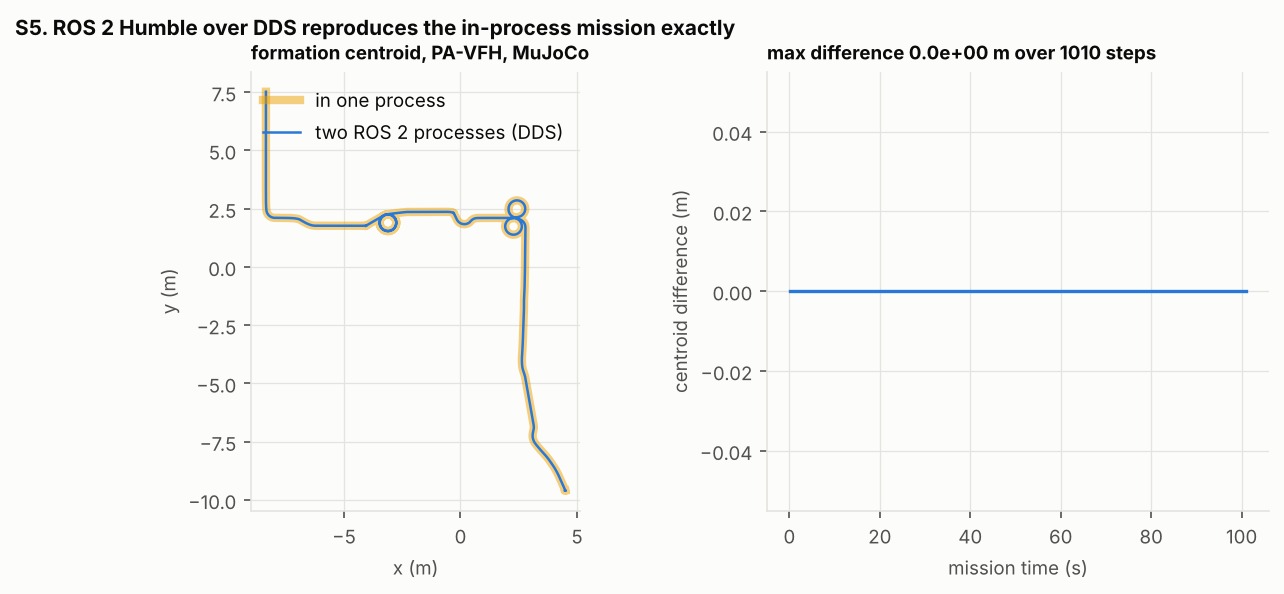
\includegraphics[width=\columnwidth]{S5_ros2_lockstep_equality.png}
\caption{The same MuJoCo mission as two ROS~2 processes over DDS and in one
process: centroid paths coincide; difference 0\,m at every step.}
\label{fig:s5}
\end{figure}

% =====================================================================
\section{Discussion}
\textit{Where learning pays.} In a pre-registered test the learned occupancy
model gives a small but significant speed-up (about 1\,\%) and is otherwise
neutral; its practical value is that \pavfh{} no longer needs the traffic plan
and still has the highest reach. The apparent reduction in gate rejections in
the smaller E19 sample did not replicate---a reminder that ablations of learned
components need confirmatory runs. The strongest learned
result is the DAgger policy, which matches its MPC teacher at about 2.5$\times$
less compute and is among the most robust in physics.

\textit{Benchmark traps.} A fixed traffic timetable, a ground-truth gate
reported as safety, and kinematics-only evaluation each flattered at least one
planner here. All three are cheap to avoid.

\textit{Kinematic vs.\ physical safety.} Laws that steer to the boundary of
what the gate admits need a physical margin; laws with an internal safety
distance already have one.

\textit{Sensor requirement.} With range noise above about 5\,cm, any monitor
with a $3\sigma$ margin closes the narrowest corridors; real-sensor reach
recovered up to $\sigma=0.05$\,m after a noise-scaled self-filter and a robust
per-beam range estimate. This is a specification for hardware, not a tuning
issue.

% =====================================================================
\section{Limitations}
All results are simulated (kinematic, MuJoCo, and ROS~2 with simulated
sensors); nothing ran on hardware. The ground-truth gate is a screening device,
not a safety system. Deployable safety is supported only by the measured
false-accept rates for this sensor model and these noise levels; the learned
monitor's conformal guarantee is marginal and in-distribution, and it needed
re-calibration for fused per-robot scans. Learned components carry no
guarantee; the gate commits every pose. Movers are constant-velocity shuttles
that never yield; no people are modelled.

% =====================================================================
\section{Conclusion}
A fair, replicated benchmark changes the conclusions one draws about local
steering for cooperative transport: the effective ingredients are simple
(range filtering, a physical margin), fixed timetables and ground-truth safety
mislead, and learning helps most when it imitates a strong planner or replaces
information a robot cannot have. \pavfh{} shows that a small learned predictor
can live inside an auditable classical pipeline and run from the robots' own
sensors through ROS~2 in physics. Code, scenarios, weights and every run are
released.

\section*{Data Availability}
All code, scenario files, configurations, trained weights and derived results,
including per-step logs of every run, are archived with SHA-256 checksums
(Zenodo DOI to be added).

\bibliographystyle{IEEEtran}
\bibliography{refs}

\end{document}
